\documentclass
   [kulak] % options: kulak (default) or kul, handout 
   {kulakbeamer}

\usepackage[dutch]{babel}
\usepackage[T1]{fontenc}
\usepackage{amsmath}
\usepackage{amssymb}
\usepackage{tabularx,array}

\title[Chapter 15: Dynamic Programming]{Chapter 15: Dynamic Programming}
\subtitle{(based on book “Introduction to Algorithms” of Cormen et al.)}
\author[]{Flor De Meulemeester} 
\institute[Kulak]{KU Leuven Kulak}
\date{Academiejaar 2024 -- 2025}

%% Overview at begin of each section; delete if unwanted.
\AtBeginSection[]{
	\begin{frame}
	\frametitle{Overzicht} %Change to "Outline" for English presentation
	{
		\hypersetup{hidelinks} %disable link colors
		\hfill	{\large\parbox{.95\textwidth}{\tableofcontents[currentsection,hideothersubsections]}}
	}
\end{frame}
}

\begin{document}

\begin{titleframe}
\titlepage
\end{titleframe}

\begin{outlineframe}[Overzicht]
\tableofcontents
\end{outlineframe}

 % % % Here you go  % % % 

\section{Inleiding}

\begin{frame}
\frametitle{Fibonacci recursief}
    \begin{itemize}
        % dynamic programming is specifiek voorbeeld van divide and conquer en vooral optimalisatie problemen waarbij er overlap is tussen subproblemen
        % en programming betekent data in array of tabel zetten 
        \item<1-> We berekenen het $n$-de Fibonacci getal
        % defenitite Fibonacci aan bord
        \item<2-> Recursief is niet efficiënt maar hoe kunnnen we het beter maken?
        % met tekening aan bord
        \item<2-> Doen we dubbel werk?
        \item<3-> Idee: Oplossingen van overlappende subproblemen opslaan
        \item<4-> Gelijkaardig met \textit{divide and conquer}
        \item<5-> Techniek vooral goed voor optimalisatie problemen (bepaalde waarde maximaliseren/minimaliseren)
    \end{itemize}
\end{frame}

\begin{frame}
\frametitle{Stappen plan voor \textit{dynamic programming}}
    \begin{enumerate}
        \item Bepaal de \textbf{structuur} van de oplossing
        \item Bepaal de \textbf{recursieve} relatie van een waarde van een oplossing t.o.v. die van de subproblemen
        \item Bereken de \textbf{waarde} van de optimale oplossing
        \item Construeer het \textbf{pad} naar de optimale oplossing
    \end{enumerate}
\end{frame}

\section{Staaf snijden}

\begin{frame}{Stap 1: Probleem voorstellen}
    \begin{itemize}
        \item<1-> Gegeven volgende tabel:
        \begin{table}[h]
            \centering
            \begin{tabular}{c|cccccccccc}
                lengte $i$ & $1$ & $2$ & $3$ & $4$ & $5$ & $6$ & $7$ & $8$ & $9$ & $10$ \\
                \hline
                prijs $p_i$ & $1$ & $5$ & $8$ & $9$ & $10$ & $17$ & $17$ & $20$ & $24$ & $30$
            \end{tabular}
        \end{table}
        \item<1-> Een stuk met lengte $i$ wordt verkocht aan prijs $p_i$
        % er is misschien meer vraag naar een stuk van specifieke lengte
        \item<2-> Verdeel staaf van lengte $n$ in $1 \leq k\leq n$ stukken zodat de prijs maximaal is
        \item<3-> De lengte is $n = i_1 + i_2 + ... + i_k$
        \item<4-> Totale prijs is $p = p_{i_1} + p_{i_2} + ... + p_{i_k}$
        \item<5-> Bijvoorbeeld: Een stuk met lengte $n = 4$ kunnen we verdelen in $2$ stukken van lengte $2$ en dus $p_2 + p_2 = 5 + 5 = 10$ is de prijs.
        % tekenen aan bord
    \end{itemize}
\end{frame}

\begin{frame}{Voorbeeld}
    Alle mogelijke onderverdelingen voor $n = 4$:
    \begin{figure}
        \centering
        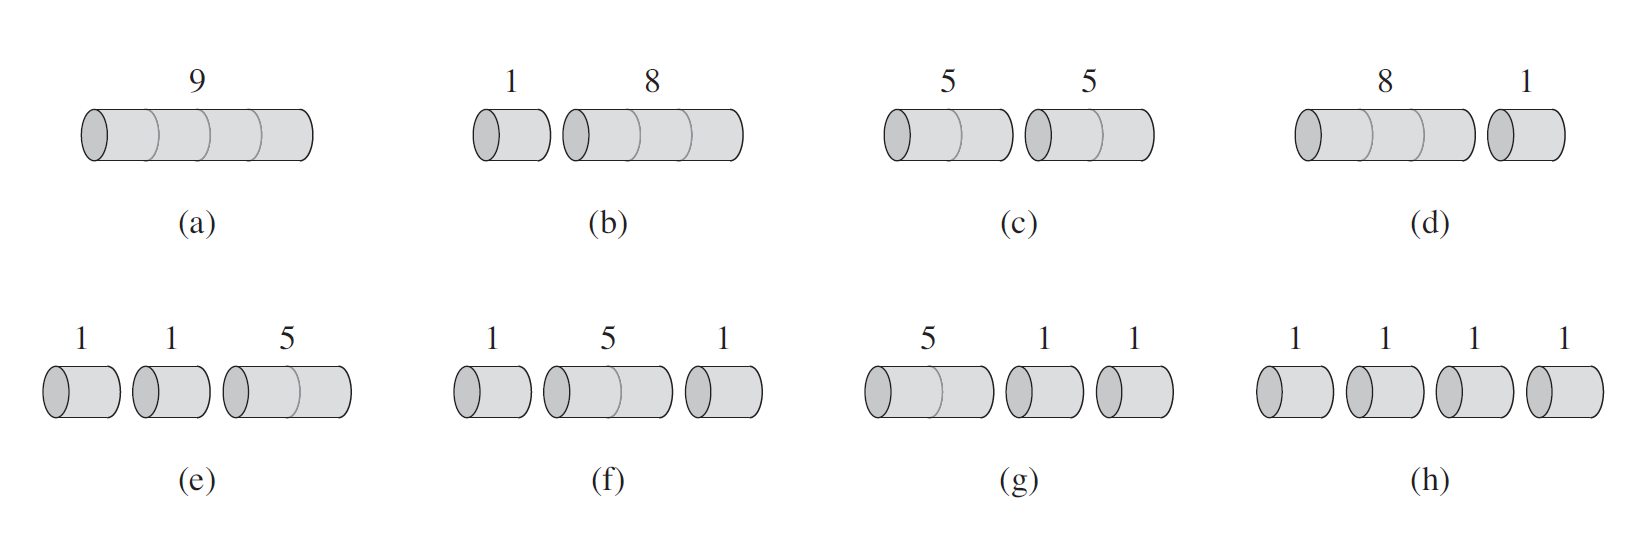
\includegraphics[width=\linewidth]{rodcuttingn4.png}
    \end{figure}  
\end{frame}

\begin{frame}{Stap 2: Recursieve oplossing}
    \begin{itemize}
        \item<1-> We kiezen een index $i$ waarop we snijden maximaal en gaan recursief voor op het deel dat over blijft.
        % met tekening aan bord
        \begin{figure}
            \centering
            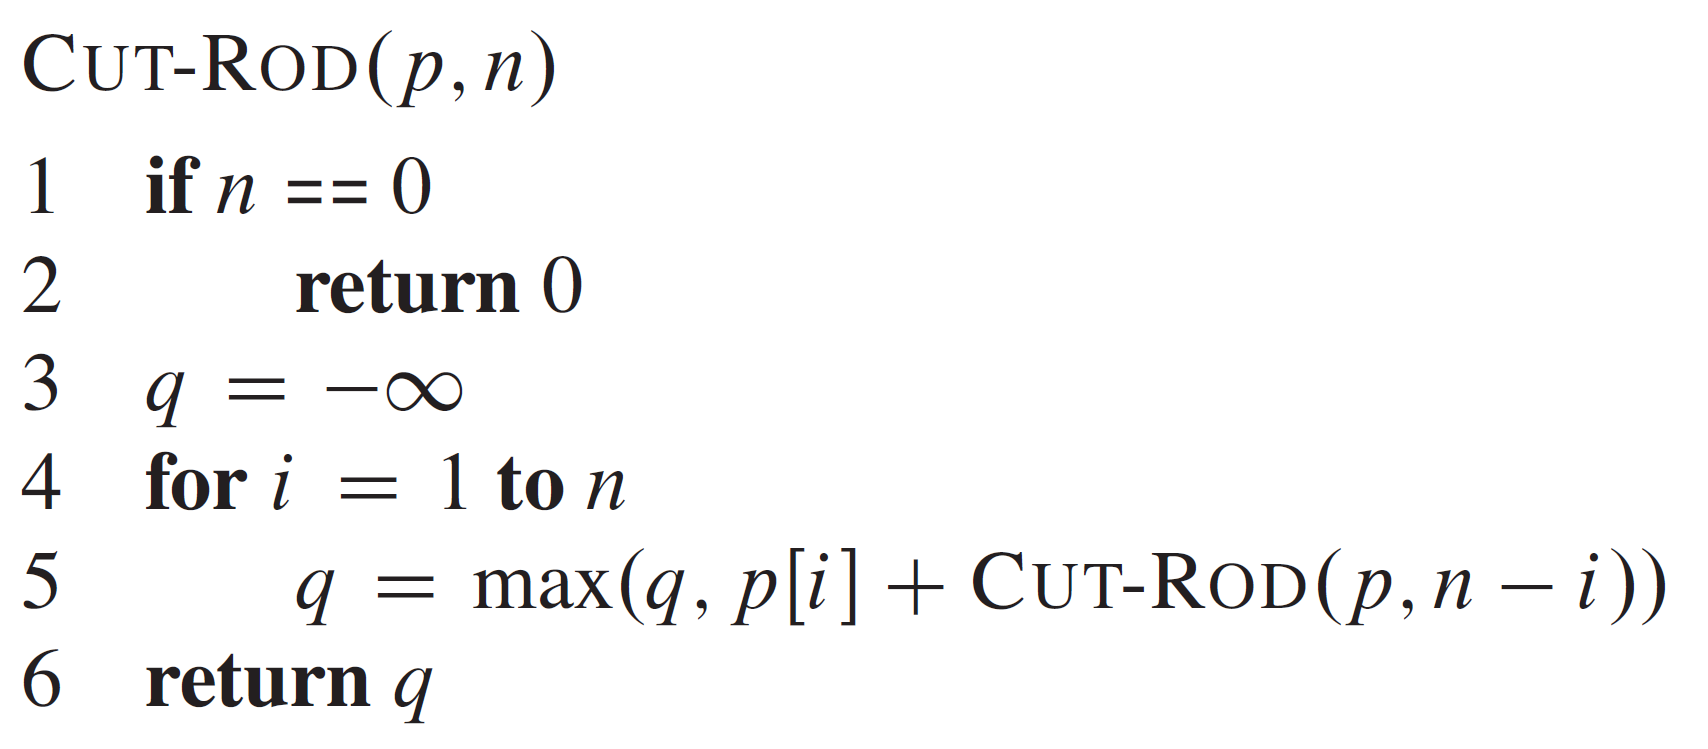
\includegraphics[width=0.6\linewidth]{naiverodcut.png}
        \end{figure}
        \item<2-> Recurrentie relatie: $T(0) = 1 \text{ en } T(n) = 1 +  \sum_{j=0}^{n-1} 1 + T(j) = 2^n$
        \item<3-> We hebben dus een algoritme met \textbf{exponentiële} uitvoeringstijd, $\mathcal{O}(2^n)$.
    \end{itemize}
\end{frame}

\begin{frame}{Recursion tree}
    \begin{figure}
        \centering
        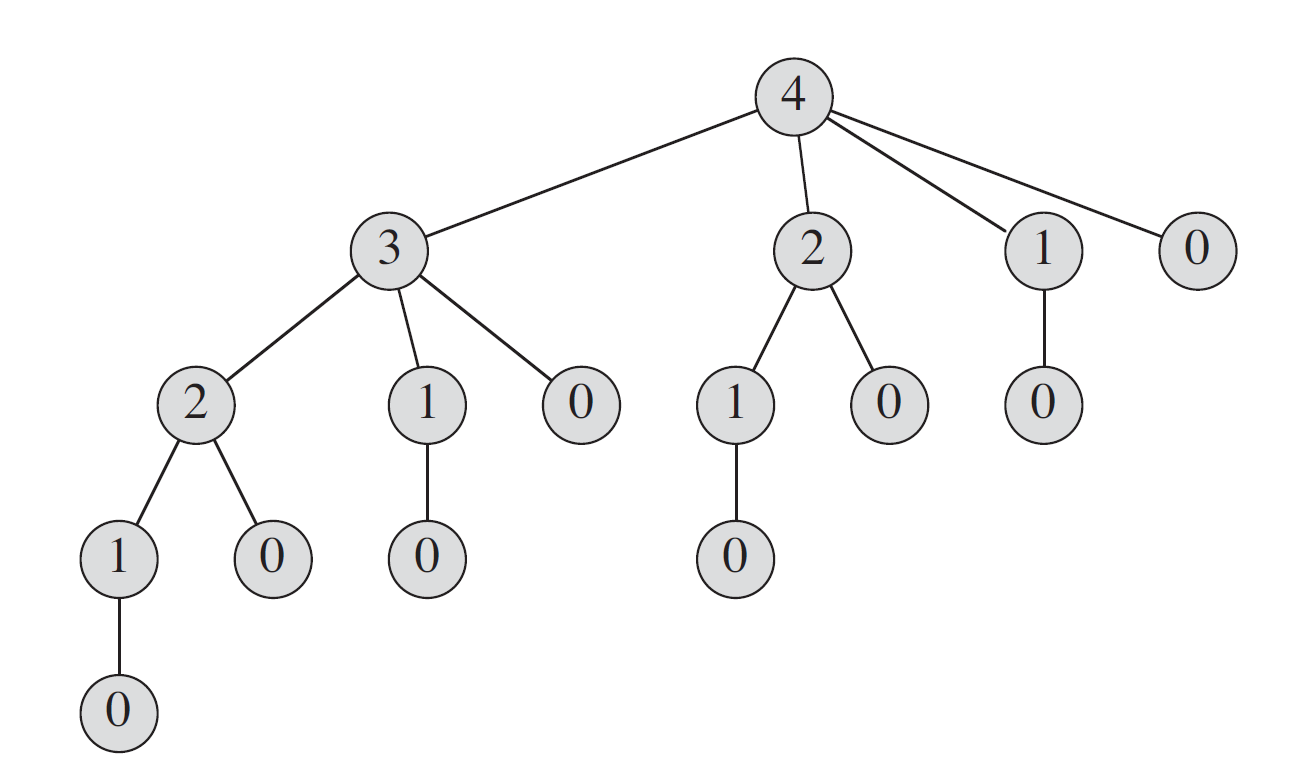
\includegraphics[width=0.7\linewidth]{recursion-tree.png}
    \end{figure}
\end{frame}

\begin{frame}{Stap 3: DP toepassen}
    \begin{itemize}
        \item<1-> DP zal in polynomiale tijd werken als er een polynomiaal aantal verschillende subproblemen bestaan.
        \item<2-> \textbf{Time-memory trade-off}
        \item<3-> We kunnen kiezen uit 2 implementaties 
        \begin{enumerate}
            % de naam zegt het zeg al een beetje (veel)
            \item \textbf{Top-down} with memoization
            \item \textbf{Bottom-up} method
        \end{enumerate}
    \end{itemize}
\end{frame}

\begin{frame}{\textbf{Top-down} implementatie}
    % voordeel indien je niet alle subproblemen nodig hebt dan zal dit beter zijn dan bottom-up
    \begin{itemize}
        \item<1-> We beginnen met ons probleem van groote $n$, als we subprobleem nodig hebben berekenen we het eenmalig en slaan het op.
        \item<2-> Idee: we hebben array (waarde ophalen in $\mathcal{O}(1)$) met de resultaten van subproblemen.
        \begin{figure}
            \centering
            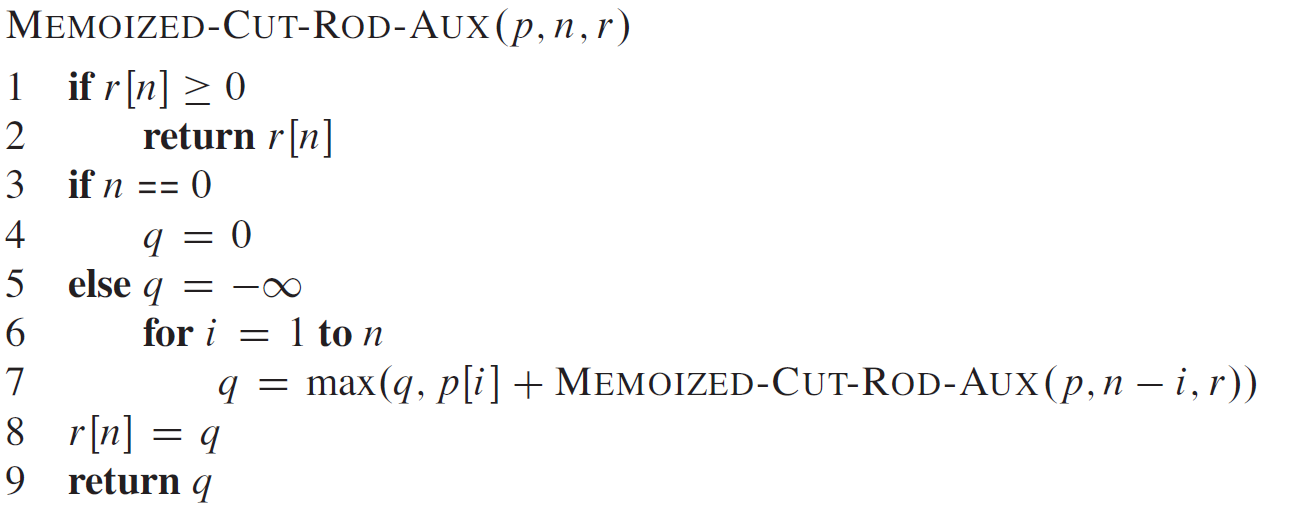
\includegraphics[width=0.75\linewidth]{topdownrodcut.png}
        \end{figure}
        \item<3-> We hebben dus een algoritme met \textbf{polynomiale} uitvoeringstijd, $\Theta(n^2)$.
    \end{itemize}
\end{frame}

\begin{frame}{\textbf{Bottom-up} implementatie}
    % indien wel alle subproblemen berekenen zal dit iets minder overhead hebben want geen recursie
    \begin{itemize}
        \item<1-> We berekenen alle subproblemen klein naar groot
        \item<2-> Opnieuw met array (waarde ophalen in $\mathcal{O}(1)$) met de resultaten van subproblemen.
        \begin{figure}
            \centering
            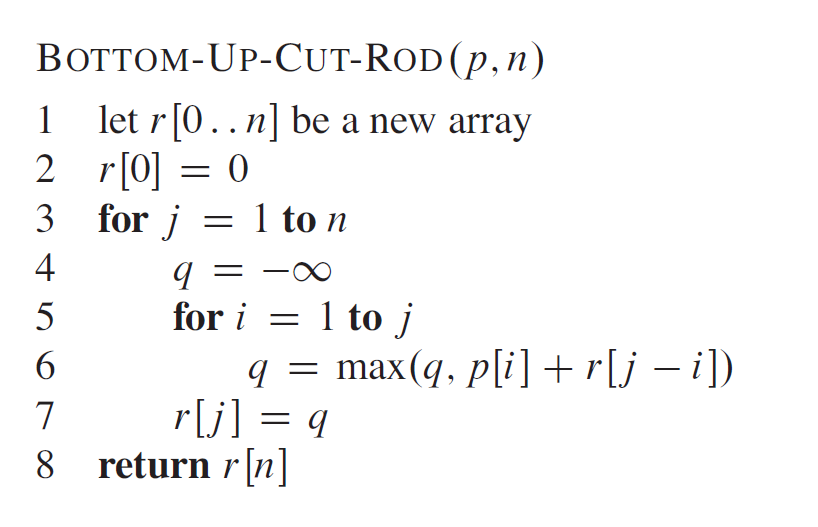
\includegraphics[width=0.5\linewidth]{bottomuprodcut.png}
        \end{figure}
        \item<3-> We hebben dus een algoritme met \textbf{polynomiale} uitvoeringstijd, $\Theta(n^2)$.
    \end{itemize}
\end{frame}

\begin{frame}{Subproblem graph}
    % je ziet voor welk probleem, welke resultaten van subproblemen we nodig hebben
    \begin{figure}
        \centering
        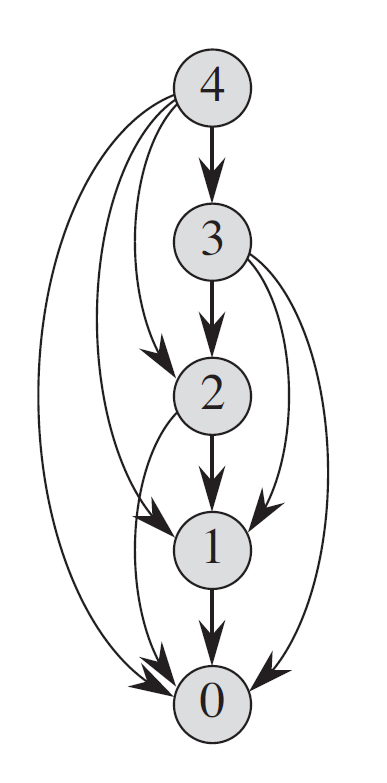
\includegraphics[width=0.2\linewidth]{subproblem-graph.png}
    \end{figure}
\end{frame}

\begin{frame}{Java implementatie}
\begin{itemize}
    \item Voor $n = 1,...,10$
\end{itemize}
\begin{figure}
    \centering
    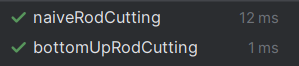
\includegraphics[width=0.9\linewidth]{java.png}
\end{figure}
\end{frame}

\begin{frame}{Stap 4: De verdeling voor de optimale waarde}
    \begin{itemize}
        \item We passen het algoritme lichtjes aan om de gemaakte stappen bij te houden.
    \end{itemize}
    \begin{columns}
        \column{.5\textwidth}
        \begin{figure}
            \centering
            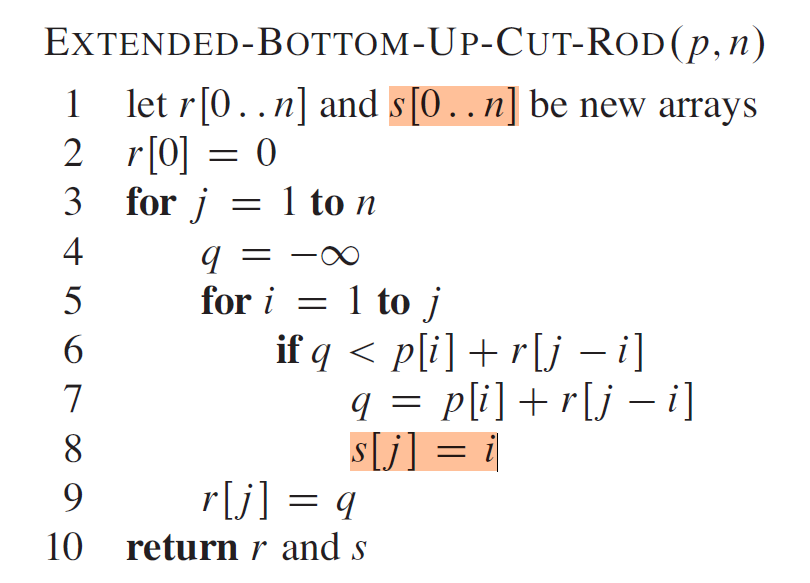
\includegraphics[width=\linewidth]{extendedbottomupcutrod.png}
        \end{figure}
        \column{.5\textwidth}
        \begin{figure}
            \centering
            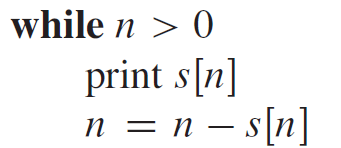
\includegraphics[width=\linewidth]{solution.png}
        \end{figure}
    \end{columns}
\end{frame}

\section{Matrix-ketting vermenigvuldigen}

\begin{frame}{Stap 1: Probleem voorstellen}
    \begin{itemize}
        \item<1-> Gegeven volgende tabel:
        \begin{table}[]
            \centering
            \begin{tabular}{c|cccccc}
                matrix & $A_1$ & $A_2$ & $A_3$ & $A_4$ & $A_5$ & $A_6$ \\
                \hline
                dimensie & $30 \times 35$ & $35 \times 15$ & $15 \times 5$ & $5 \times 10$ & $10 \times 20$ & $20 \times 25$
            \end{tabular}
        \end{table}
        \item<2-> Matrices niet commutatief wel associatief, we willen haakjes zo efficiënt mogelijk zetten zodat we minimaal aantal scalair vermenigvuldigingen moeten berekenen.
        \item<3-> Voor een matrix van $p \times q$ en een matrix $q \times r$ is dit $pqr$ aantal bewerkingen.
        \end{itemize}
\end{frame}

\begin{frame}{Voorbeeldje}
    \begin{columns}
        \column{.5\textwidth}
        \begin{itemize}
            \item<1-> \begin{center} $A_1  A_2  A_3  A_4$ \end{center}
        \end{itemize}
        Mogelijkheden:
        \begin{itemize}
            \item<2-> $(A_1(A_2(A_3A_4)))$
            \item<2-> $(A_1((A_2A_3)A_4))$
            \item<2-> $((A_1A_2)(A_3A_4))$
            \item<2-> $((A_1(A_2A_3))A_4)$
            \item<2-> $(((A_1A_2)A_3)A_4)$
        \end{itemize}
        \column{.5\textwidth}
        \begin{itemize}
            \item<3-> $P(n) = \#$ mogelijkheden voor $n$
            \begin{align*}
                & P(1) = 1  \\
                & P(n) = \sum_{k=1}^{n-1} P(k)P(n-k) \text{ met } n \geq 2
            \end{align*}
            \item<4-> $1, 1, 2, 5, 14, 42, 132, 429, 1430, 4862, ...$ \\
            \item<5-> De Catalan-getallen groeien met $\Omega(4^n/n^\frac{3}{2})$
        \end{itemize}
    \end{columns}
\end{frame}

\begin{frame}{Stap 2: Recursieve oplossing}
\begin{itemize}
    \item<1-> We zullen een subprobleem $A_iA_{i+1}...A_j$ als volgt opsplitsen in 2 nieuwe subproblemen $A_iA_{i+1}...A_k$ en $A_{k+1}A_{k+2}...A_j$.
    \item<2-> We zetten haakjes achter $A_k$
    \item<3-> De oplossingen van deze subproblemen zullen we bijhouden in een $n \times n$ matrix $m$. De oplossing voor $A_iA_{i+1}...A_{j-1}A_j$ vinden we dan in $m[i,j]$.
    \item<4-> $m[i,i] = 0$
    \item<5-> De naïeve recursieve oplossing zal opnieuw \textbf{exponentiële} uitvoeringstijd hebben.
\end{itemize}
\end{frame}

\begin{frame}{Stap 3: DP toepassen}
\begin{figure}
    \centering
    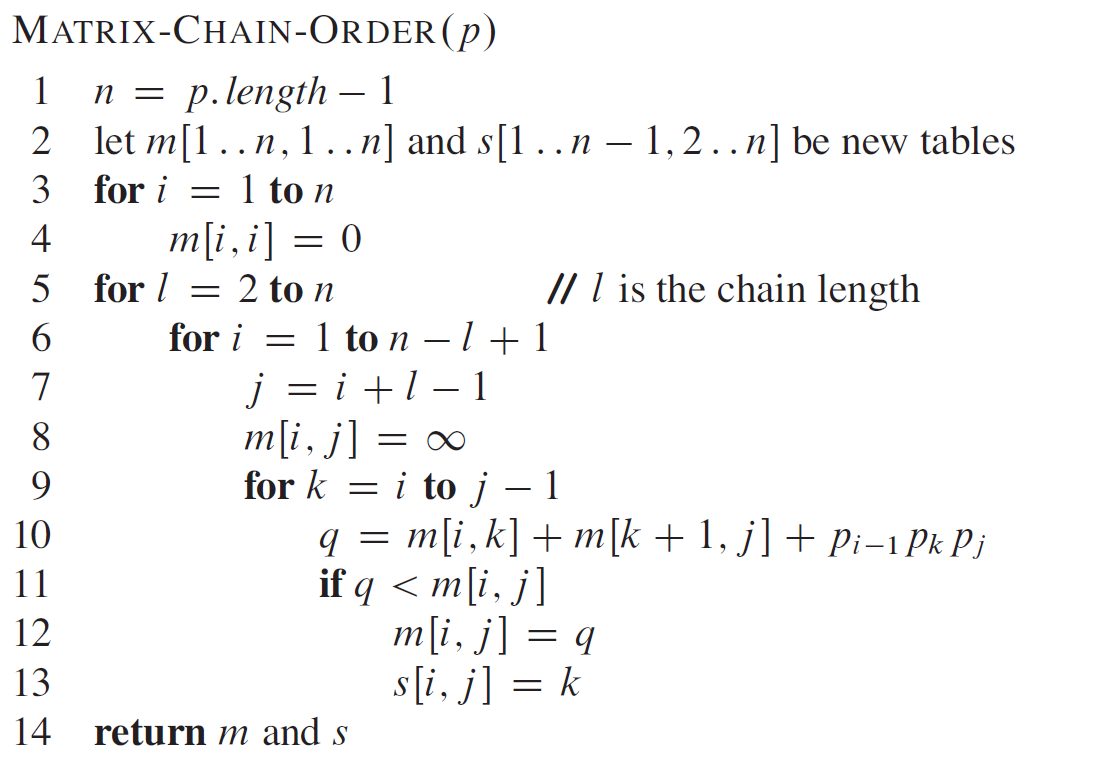
\includegraphics[width=0.55\linewidth]{matrixchain.png}
    \begin{itemize}
        \item<1-> Complexiteit: $\mathcal{O}(n^3)$
    \end{itemize}
\end{figure}
\end{frame}

\begin{frame}{Matrices m and s}
\begin{itemize}
    \item \textbf{Bottom-up} voor elke $l$ de optimale oplossing berekenen voor verschillende matrices.
\end{itemize}
\begin{figure}
    \centering
    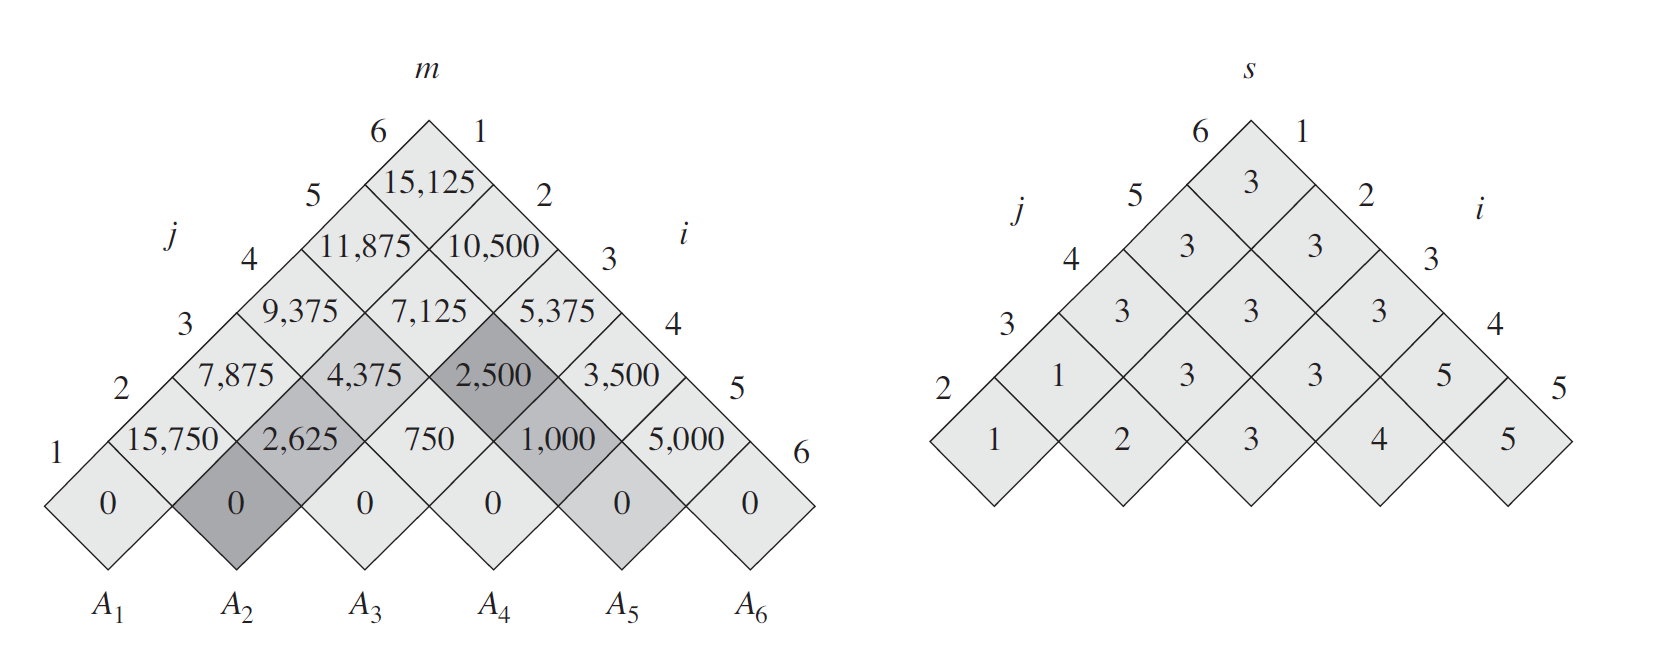
\includegraphics[width=0.8\linewidth]{mands.png}
\end{figure}
\end{frame}

\begin{frame}{Stap 4: Optimale haakjes}
\begin{itemize}
    \item In $s$ houden we bij op welke $k$ we optimaal gesplitst hebben.
    \item Zo kunnen we de oplossing reconstrueren.
\end{itemize}
\begin{figure}
    \centering
    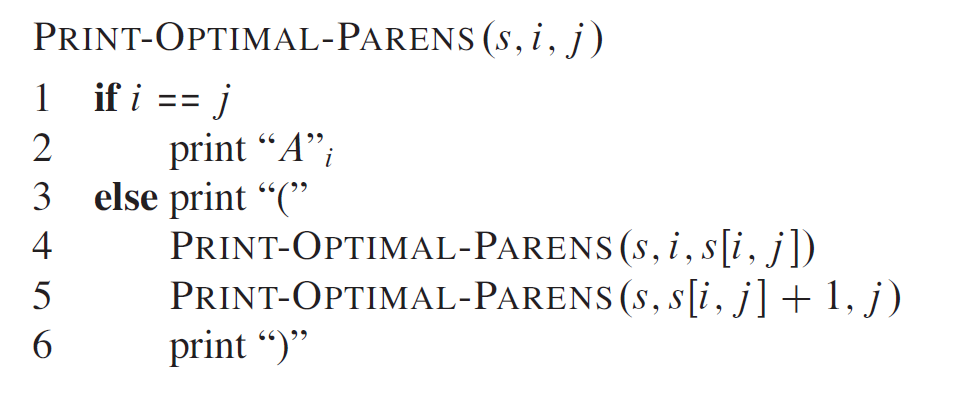
\includegraphics[width=0.7\linewidth]{printsolutions.png}
\end{figure}
\end{frame}

\section{Voorwaarden voor \textit{dynamic programming}}
\begin{frame}{Eigenschap 1: Optimale substructuur}
\begin{itemize}
    \item<1-> Als de optimale oplossing vervat zit in de optimale oplossing van de subproblemen.
    \item<2-> Vaak complexiteit van de vorm $\mathcal{O}(n^{a + b})$
    \begin{itemize}
        \item<2-> $a = $ \# subproblemen per probleem
        \item<3-> $b = $ \# keuzes per subprobleem
    \end{itemize}
\end{itemize}
\end{frame}

\begin{frame}{Subproblemen moet onafhankelijk zijn}
\begin{columns}
    \column{.6\textwidth}
    \begin{itemize}
        \item<1-> $q \xrightarrow{} r$ en $r \xrightarrow{} t$ zijn subproblemen van $q \xrightarrow{} t$
        \item<2-> Ongewogen kortste pad
        \begin{itemize}
            \item<2-> $q \xrightarrow{} r$
            \item<2-> $r \xrightarrow{} t$
        \end{itemize}
        \item<3-> Ongewogen langste \textbf{simpel} pad
        \begin{itemize}
            \item<4-> $q \xrightarrow{} s \xrightarrow{} t \xrightarrow{} r$
            \item<5-> $r \xrightarrow{} q \xrightarrow{} s \xrightarrow{} t$
            \item<6-> Pad is niet meer simpel
        \end{itemize}
    \end{itemize}
    \column{.4\textwidth}
    \begin{figure}
        \centering
        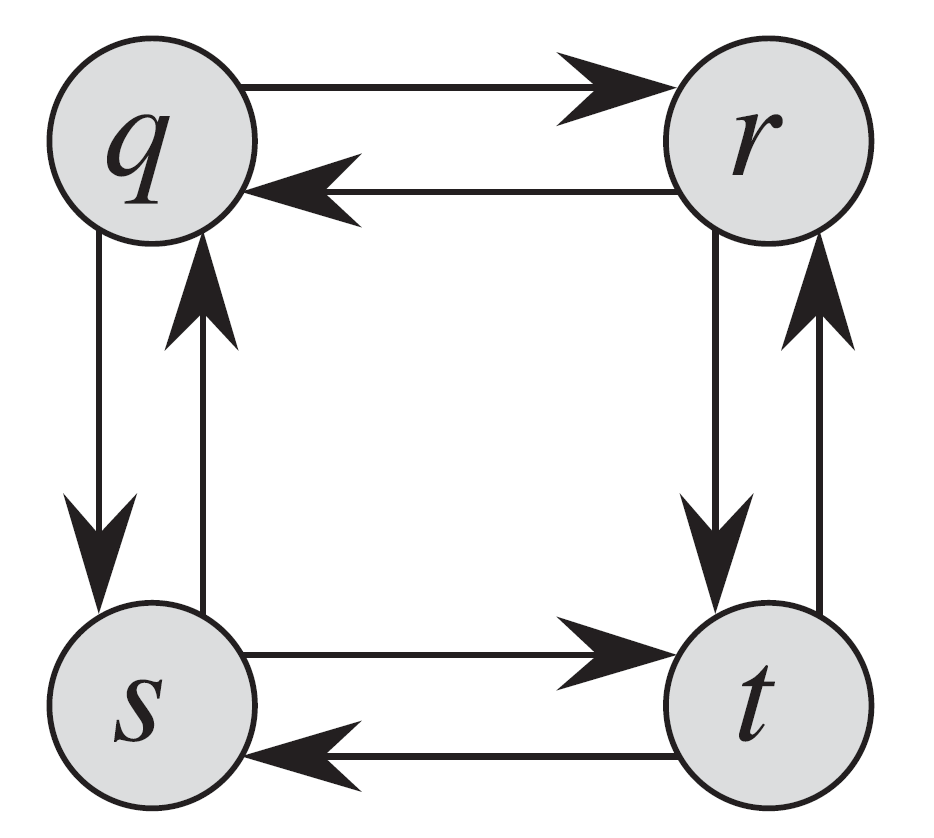
\includegraphics[width=\linewidth]{graph.png}
    \end{figure}
\end{columns}
\end{frame}

\begin{frame}{Eigenschap 2: Overlappende subproblemen}
\begin{itemize}
    \item<1-> Het matrix probleem heeft ook overlappende problemen
    \item<2-> Polynomiaal \#verschillende subproblemen
\end{itemize}
\begin{figure}
    \centering
    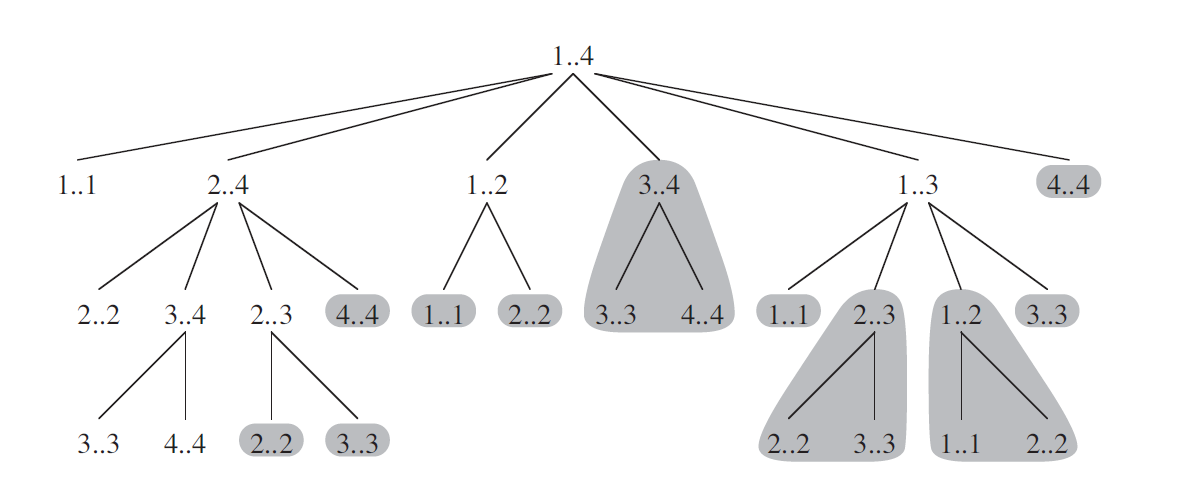
\includegraphics[width=0.8\linewidth]{recursivematrix.png}
\end{figure}
\end{frame}

\section*{Vragen}
\begin{frame}{Vragen}
    Zijn er nog vragen?
    % Verschil met greedy algoritms:
    % DP takes an informed choice
    % GA takes the choice that looks best at the time so don't go over all the choices (sometimes better, sometimes not)
\end{frame}

\end{document}